


\documentclass[
a4paper,        % A4 papier
headsepline,    % Kopfzeile
footsepline     % Fusszeile
]{scrartcl}

\usepackage[T1]{fontenc}
\usepackage[utf8]{inputenc}
\usepackage[english]{babel}
\usepackage{mathpazo}


\usepackage{blindtext}
\usepackage{url}
\usepackage{caption}
\usepackage{subcaption}
\usepackage{placeins}
\usepackage{units}
\usepackage{amssymb}
\usepackage{amsmath} % Required for some math elements 
\usepackage{graphicx} % Required for the inclusion of images

\usepackage{paralist}                               % Listen mit speziellen Identifiern
\usepackage{mdwlist}                                % Listen ohne Zwischenzeilenabstand



% My commands
\newcommand{\myemph}[1]{ \emph{#1} }



% My Theorems
\newtheorem{bsp}{Beispiel}
\newtheorem{theo}{Theorem}
\newtheorem{defi}{Definition}
\newtheorem{koro}{Korollar}
\newtheorem{lemma}{Lemma}
\newtheorem{algo}{Algorithmus}
\newtheorem{bew}{Beweis}





\setcounter{secnumdepth}{2}                         % Numerierungtiefe
\hyphenation{}




\pagestyle{plain}
\pagenumbering{arabic}







\begin{document}

\title{TMA4280 -- Project 1}
\author{Maximilian Kieler}
\date{\today}

\maketitle


\section{Introduction}

Aim of the Project is to implement an algorithm to sum a series in a serial way and in parallel by using MPI and OpenMP. The exact tasks and further specifications can be found in \cite{}. In reason that my access to Lille does not work\footnote{It worked weeks ago, but now all my jobs land on the queue and remain there and do not get accepted.} the analysis of the parallel implementation is not possible or at least only on my own computer\footnote{Intel i5}.  




\section{Serial Implementation}

It is task to implement a serial method to find the solution of two sums. Therefore we use the language c++. The implementation is done in an object oriented style and uses the template mechanism, which make it possible to use the same basic class for both sums. We provide a method to solve the sum and print the result. Furthermore there exists a unit test, which prints the error of the result to the original value for a sum over three terms. Finally there exists a verification test, which gives the error in dependence to the number of summed terms. As we see in Fig.~\ref{fig:convergence_series}\begin{figure}[h] 
  \centering
     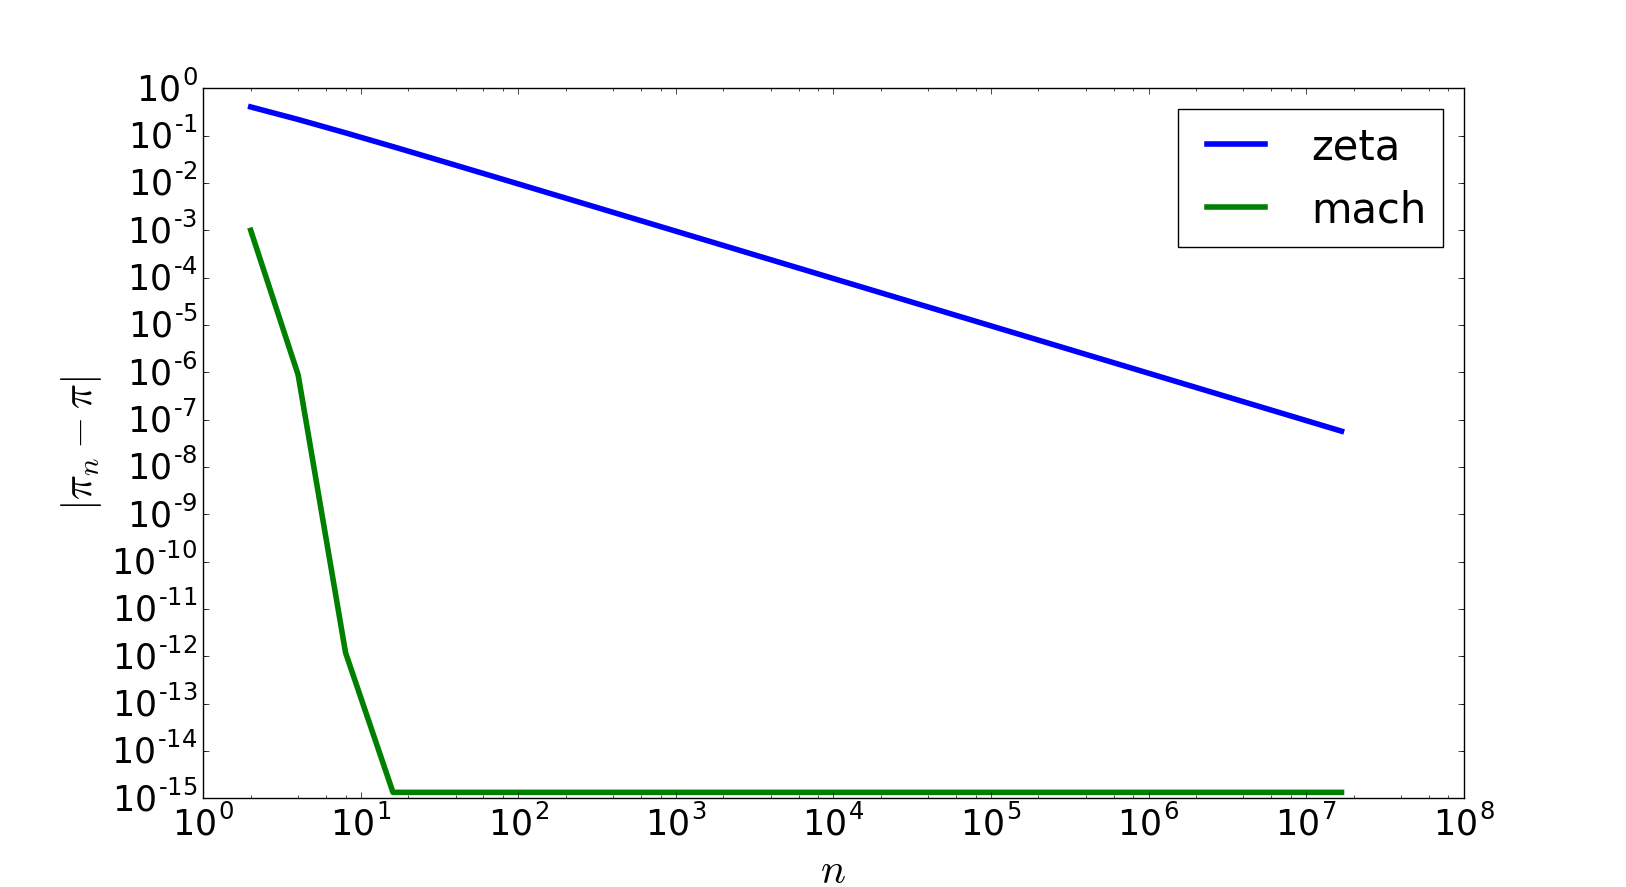
\includegraphics[width=\textwidth]{pic/convergence_series.png}
  \caption{The convergence of the zeta series is worse than the mach series. This series converge after four terms to machine precision. The use of a big number of terms is here useless and parallelisation not necessary. However the worse convergence of the zeta series make it necessary to use many terms to get a good result.}
  \label{fig:convergence_series}
\end{figure} the convergence of series $2$ is better than of series $1$. Less terms are needed to get the most exact result which is possible on a computer with double precision. 






\section{MPI Implementation}

The implementation should be done in the way, that we allocate a vector, fill it with the values of the terms and distribute the to the processes. This is not really a suitable solution to the problem in the way that we allocate an possibly big array, but we need the values only once. The summation can be done immediately after evaluating the terms, but however, the task is written to practice the MPI mechanism. To avoid the allocation of a big array in the root process, we decided to allocate only a array of the size of the distributed array and fill this in the loop before sending. This leads to a slight deparallelisation and is only suggestive if the filling process takes not to much time. The program measure the wall time by using the MPI wall time function. As we are interested in the execution time of the program we start the measurement in the root process and stop it there after all processes have returned their results and added together. We can not expect, that the result of the MPI implementation is completely the same as for the serial implementation. There we add a small number to a number of a much higher magnitude. Due to floating number calculation this results in errors. In the MPI implementation we calculate local all small numbers of the same magnitude, so the reach possibly a higher magnitude and add this partial sums afterwards. Therefore this result can be more precise. But this is only a theoretical objection. In reason of the equal sized distribution such effects does no occur. We observe the same error for $P=2$ and $P=8$. It should be mention, that for the mach series the summation of terms below the machine precision yields an additional error which should be avoided. 


\section{OMP Implementation}

We use OpenMP in the way the we parallize the loop which fills the vector. This operation is completely load balanced, so no further options are necessary. The second addition is done by parallize the loop which sums the vector by using the OpenMP reduction. These two simple additions can also be added in the MPI implementation. 

\section{Conclusion}

As previous said, the way of implementing the problem by first filling a vector is not efficient. The number of FLOPs for filling a vector of size n is given by $\text{FLOP}(\text{fill}) = n \cdot \text{FLOP}(\text{eval})$ (if we assume that assignment is also a FLOP), where $\text{FLOP}(\text{eval})$ is the number of FLOPS needed to evaluate one term of the series. The summation over the vector consists in assign the value, add it, and assign the result, which gives us $3n$ FLOPs. More efficient is to collapse the two loops and do the summation immediately. Nevertheless the way of the implementation is perfectly load balanced if the number of terms is a multiple of the number of processes. This is in reason of simplicity the only allowed case in the implementation. Otherwise the will be one process which only have to sum over $n - n \% (P-1)$ remaining terms. However the use of parallelism is for this problem not necessary. We have seen that the zeta series converges slowly, so many terms are needed, here it could make seens to parallize the loop, but it is much easier to use the mach series which converges after 4 terms to machine precision. For a loop over 4 terms the overhead to organize the parallel environment is much more time expensive as to compute it in serial. To solve this problem in parallel is only useful as an exercise for learning purpose. 





\end{document}